%Fred's NSF Grant Dec 2017
\documentclass[11pt]{NSFamsart}
\usepackage{latexsym,amsfonts,amsmath,epsfig,multirow}
\usepackage{stackrel,tabularx,mathtools,enumitem,xspace}
\usepackage[dvipsnames]{xcolor}
\usepackage[numbers]{natbib}
\usepackage{hyperref,accents}
\usepackage{algorithm, algorithmic}
\usepackage{cleveref}
\newcommand\myshade{85}
\colorlet{mylinkcolor}{violet}
\colorlet{mycitecolor}{Aquamarine}
%\colorlet{mycitecolor}{OliveGreen}
\colorlet{myurlcolor}{YellowOrange}

\hypersetup{
	linkcolor  = mylinkcolor!\myshade!black,
	citecolor  = mycitecolor!\myshade!black,
	urlcolor   = myurlcolor!\myshade!black,
	colorlinks = true,
}


% This package prints the labels in the margin
%\usepackage[notref,notcite]{showkeys}


%\pagestyle{empty}
\thispagestyle{plain}
\pagestyle{plain}

\headsep-0.6in
%\headsep-0.45in

\setlength{\textwidth}{6.5in}
\setlength{\oddsidemargin}{0in}
\setlength{\evensidemargin}{0in}
\textheight9in
%\textheight9.1in

\providecommand{\FJHickernell}{Hickernell}
\newcommand{\hI}{\hat{I}}
\newcommand{\hatf}{\hat{f}}
\newcommand{\hatg}{\hat{g}}
\newcommand{\tf}{\tilde{f}}
\newcommand{\tbf}{\tilde{\bff}}
%\DeclareMathOperator{\Pr}{\mathbb{P}}
\DeclareMathOperator{\cost}{cost}
\DeclareMathOperator{\loss}{loss}
\DeclareMathOperator{\lof}{lof}
\DeclareMathOperator{\reg}{reg}
\DeclareMathOperator{\CV}{CV}
\DeclareMathOperator{\size}{wd}

\def\reals{{\mathbb{R}}}
\def\field{{\mathbb{F}}}
\def\complex{{\mathbb{C}}}
\def\naturals{{\mathbb{N}}}
\def\integer{{\mathbb{Z}}}
\def\expect{{\mathbb{E}}}
\def\il{\left<}
\def\ir{\right>}
\def\e{\varepsilon}
\def\g{\gamma}
\def\l{\lambda}
\def\b{\beta}
\def\a{\alpha}
\def\lall{\Lambda^{{\rm all}}}
\def\lstd{\Lambda^{{\rm std}}}

\newcommand{\hV}{\widehat{V}}
\newcommand{\tV}{\widetilde{V}}
\newcommand{\hcut}{\frak{h}}

\newcommand{\bbE}{\mathbb{E}}
\newcommand{\tQ}{\widetilde{Q}}
\newcommand{\mA}{\mathsf{A}}
\newcommand{\mB}{\mathsf{B}}
\newcommand{\mC}{\mathsf{C}}
\newcommand{\mD}{\mathsf{D}}
\newcommand{\mG}{\mathsf{G}}
\newcommand{\mH}{\mathsf{H}}
\newcommand{\mI}{\mathsf{I}}
\newcommand{\mK}{\mathsf{K}}
\newcommand{\tmK}{\widetilde{\mathsf{K}}}
\newcommand{\mL}{\mathsf{L}}
\newcommand{\mM}{\mathsf{M}}
\newcommand{\mP}{\mathsf{P}}
\newcommand{\mQ}{\mathsf{Q}}
\newcommand{\mR}{\mathsf{R}}
\newcommand{\mX}{\mathsf{X}}
\newcommand{\mPhi}{\mathsf{\Phi}}
\newcommand{\mPsi}{\mathsf{\Psi}}
\newcommand{\mLambda}{\mathsf{\Lambda}}

\DeclareMathOperator{\err}{err}
\DeclareMathOperator{\oerr}{\overline{\err}}
\DeclareMathOperator{\herr}{\widehat{\err}}

%\DeclareMathOperator{\Spl}{Spline}
%\DeclareMathOperator{\SSpl}{SmSpline}
%\DeclareMathOperator{\Power}{Power}
%\DeclareMathOperator{\RegSpl}{RegSpline}
%\DeclareMathOperator{\MLS}{MLS}
%\DeclareMathOperator*{\argmin}{argmin}
%\DeclareMathOperator*{\rms}{rms}
%\DeclareMathOperator*{\RMSE}{RMSE}
%\DeclareMathOperator*{\bias}{bias}
%\DeclareMathOperator*{\var}{var}
\DeclareMathOperator{\Var}{Var}
\DeclareMathOperator{\INT}{INT}
\DeclareMathOperator{\APP}{APP}
\DeclareMathOperator{\OPT}{MIN}

\newcommand{\bone}{\boldsymbol{1}}
\newcommand{\bzero}{\boldsymbol{0}}
\newcommand{\binf}{\boldsymbol{\infty}}
\newcommand{\ba}{{\boldsymbol{a}}}
\newcommand{\bb}{{\boldsymbol{b}}}
\newcommand{\bc}{{\boldsymbol{c}}}
\newcommand{\bd}{{\boldsymbol{d}}}
\newcommand{\be}{{\boldsymbol{e}}}
\newcommand{\bff}{{\boldsymbol{f}}}
\newcommand{\bhh}{{\boldsymbol{h}}}
\newcommand{\beps}{{\boldsymbol{\varepsilon}}}
\newcommand{\tbeps}{\tilde{\beps}}
\newcommand{\bx}{{\boldsymbol{x}}}
\newcommand{\bX}{{\boldsymbol{X}}}
\newcommand{\bh}{{\boldsymbol{h}}}
\newcommand{\bk}{{\boldsymbol{k}}}
\newcommand{\bg}{{\boldsymbol{g}}}
\newcommand{\bv}{{\boldsymbol{v}}}
\newcommand{\bu}{{\boldsymbol{u}}}
\newcommand{\by}{{\boldsymbol{y}}}
\newcommand{\bt}{{\boldsymbol{t}}}
\newcommand{\bz}{{\boldsymbol{z}}}
\newcommand{\bvarphi}{{\boldsymbol{\varphi}}}
\newcommand{\bgamma}{{\boldsymbol{\gamma}}}
\newcommand{\bphi}{{\boldsymbol{\phi}}}
\newcommand{\bpsi}{{\boldsymbol{\psi}}}
\newcommand{\bnu}{{\boldsymbol{\nu}}}
\newcommand{\balpha}{{\boldsymbol{\alpha}}}
\newcommand{\bbeta}{{\boldsymbol{\beta}}}
\newcommand{\bo}{{\boldsymbol{\omega}}}  %GF added
\newcommand{\newton}[2]{\left(\begin{array}{c} #1\\ #2\end{array}\right)}
\newcommand{\anor}[2]{\| #1\|_{\mu_{#2}}}
\newcommand{\satop}[2]{\stackrel{\scriptstyle{#1}}{\scriptstyle{#2}}}
\newcommand{\setu}{{\mathfrak{u}}}

\newcommand{\me}{\textup{e}}
\newcommand{\mi}{\textup{i}}
\def\d{\textup{d}}
\def\dif{\textup{d}}
\newcommand{\cc}{\mathcal{C}}
\newcommand{\cb}{\mathcal{B}}
\newcommand{\cl}{L}
\newcommand{\cx}{{\Omega}}
\newcommand{\calc}{{\mathcal{C}}}
\newcommand{\calf}{{\mathcal{F}}}
\newcommand{\calfd}{{\calf_d}}
\newcommand{\calh}{{\mathcal{H}}}
\newcommand{\tcalh}{{\widetilde{\calh}}}
\newcommand{\calI}{{\mathcal{I}}}
\newcommand{\calhk}{\calh_d(K)}
\newcommand{\calg}{{\mathcal{G}}}
\newcommand{\calgd}{{\calg_d}}
\newcommand{\cL}{\mathcal{L}}
\newcommand{\cP}{\mathcal{P}}
\newcommand{\cT}{\mathcal{T}}
\newcommand{\cK}{\mathcal{K}}
\newcommand{\fA}{\mathfrak{A}}
\newcommand{\fC}{\mathfrak{C}}
\newcommand{\fF}{\mathfrak{F}}
\newcommand{\fL}{\mathfrak{L}}
\newcommand{\hS}{\widehat{S}}
\DeclareMathOperator{\Prob}{\mathbb{P}}

\def\abs#1{\ensuremath{\left \lvert #1 \right \rvert}}
\newcommand{\bigabs}[1]{\ensuremath{\bigl \lvert #1 \bigr \rvert}}
\newcommand{\norm}[2][{}]{\ensuremath{\left \lVert #2 \right \rVert}_{#1}}
\newcommand{\ip}[3][{}]{\ensuremath{\left \langle #2, #3 \right \rangle_{#1}}}
\newcommand{\bignorm}[2][{}]{\ensuremath{\bigl \lVert #2 \bigr \rVert}_{#1}}
\newcommand{\calm}{{\mathfrak{M}}}
\DeclareMathOperator{\diag}{diag}
\DeclareMathOperator{\dist}{dist}
\DeclareMathOperator{\filldis}{fill}
\DeclareMathOperator{\sep}{sep}
\DeclareMathOperator{\avg}{avg}
\DeclareMathOperator{\vol}{vol}
\DeclareMathOperator{\cov}{cov}

\newcommand{\des}{\{\bx_i\}}
\newcommand{\desinf}{\{\bx_i\}_{i=1}^{\infty}}
\newcommand{\desn}{\{\bx_i\}_{i=1}^n}
\newcommand{\wts}{\{g_i\}_{i=1}^N}
\newcommand{\wtsn}{\{g_i\}_{i=1}^N}
\newcommand{\datan}{\{y_i\}_{i=1}^N}

%FJH added
\newcommand{\Order}{\mathcal{O}}
\newcommand{\ch}{\mathcal{H}}
\newcommand{\tch}{{\widetilde{\ch}}}
\newcommand{\veps}{\boldsymbol{\varepsilon}}
\DeclareMathOperator{\best}{best}
\newcommand{\hmu}{\hat{\mu}}
\newcommand{\hsigma}{\hat{\sigma}}
\newcommand{\tK}{\widetilde{K}}
\newcommand{\Matlab}{{\sc Matlab}\xspace}
\newcommand{\abstol}{\varepsilon_{\text{a}}}
\newcommand{\reltol}{\varepsilon_{\text{r}}}

\newcommand\starred[1]{\accentset{\star}{#1}}


\definecolor{MATLABOrange}{rgb}{0.85,  0.325, 0.098}

\newtheorem{resproblem}{Research Problem}
\newtheorem{research}{Research Objectives}


\newcommand{\refproba}{\hyperref[SectHSSVD]{Research Project~1}\xspace}
\newcommand{\refprobaa}{\hyperref[AnalyticEigensubsec]{Research Project~1.1}\xspace}
\newcommand{\refprobab}{\hyperref[NumerEigensubsec]{Research Project~1.2}\xspace}
\newcommand{\refprobac}{\hyperref[SectDesignerKernels]{Research Project~1.3}\xspace}

\newcommand{\refprobb}{\hyperref[SectGAIL]{Research Project~2}\xspace}
\newcommand{\refprobba}{\hyperref[Integrationsubsec]{Research Project~2.1}\xspace}
\newcommand{\refprobbb}{\hyperref[Higherordersubsec]{Research Project~2.2}\xspace}

\newcommand{\refprobc}{\hyperref[combinesec]{Research Project~3}\xspace}
\newcommand{\refprobca}{\hyperref[errestsubsec]{Research Project~3.1}\xspace}
\newcommand{\refprobcb}{\hyperref[parestsubsec]{Research Project~3.2}\xspace}
\newcommand{\refprobcc}{\hyperref[designsubsec]{Research Project~3.3}\xspace}

\newcommand{\refprobd}{\hyperref[appsec]{Research Project~4}\xspace}
\newcommand{\refprobda}{\hyperref[PDEsubsec]{Research Project~4.1}\xspace}
\newcommand{\refprobdb}{\hyperref[SectMEEG]{Research Project~4.2}\xspace}
\newcommand{\refprobdc}{\hyperref[ebolasubsec]{Research Project~4.3}\xspace}
\newcommand{\refprobdd}{\hyperref[Sec_TruncHS]{Research Project~4.4}\xspace}


%\setcounter{page}{1}

\setlist[description]{font=\normalfont\itshape}



\begin{document}
%\setlength{\leftmargini}{2.5ex}

\centerline{\Large \bf Project Description}
\vspace{-2ex}

\setcounter{tocdepth}{1}
\tableofcontents

\vspace{-6ex}

\section{Scientific Context and Timeliness of the Proposed Research}
Traditional error analysis for numerical algorithms \emph{does not} support the 
stopping criteria employed by common adaptive numerical algorithms.  We will develop 
rigorous data-driven error bounds that will underpin new adaptive 
numerical algorithms for integration, function approximation, and optimization.  These 
algorithms will allow the user to expend 
the required computational effort to meet user-specified error criteria without having to 
know the norm of the input function.  
These adaptive algorithms will be 
implemented 
in the freely available GAIL software library.  They will be tested on various applications 
problems to ensure that theory matches practice.

\subsection{An Illustrative Example: Integration by the Trapezoidal Rule}  We introduce some 
of the concepts arising in our proposed research via the problem of univariate integration.  Calculus 
students are 
taught to approximate the definite integral by the trapezoidal rule 
\cite[Sect.\ 7.2, (7.15)]{BraPet11a}:
\begin{gather}
\label{traprule}
\int_0^1 f(x) \, \dif x \approx T_n(f):= \frac1{2n} \left[f(0) + 2f(1/n) + \cdots + 2f(1-1/n) + f(1) \right ], \\
\label{traperrbd}
\err_n(f) := \abs{\int_0^1 f(x) \, \dif x - T_n(f)}  \le \frac{\Var(f')}{8 n^2} =: \oerr_n(f),
\end{gather}
where the total variation of the first derivative is defined as 
\begin{equation*}
\Var(f') : = \max \left \{\widehat{V}(f',\{t_i\}_{i=0}^n) := \sum_{i=2}^{n-1}  \abs{f'(t_i) - f'(t_{i-1})} \, \Big 
\vert \, 
\forall \text{ partitions }  \{t_i\}_{i=0}^n \text{ of } [0,1], \ \forall n \in \naturals \right \}.
\end{equation*} 
A partition $\{t_i\}_{i=0}^n$ of an interval is an ordered subset of that interval including both 
endpoints.
The practitioner wants to know how large $n$ 
must be to ensure that $\err_n(f)  \le \varepsilon$, for a prescribed 
absolute error tolerance $\varepsilon$.  Ensuring that $\oerr_n(f) \le \varepsilon$ is sufficient, but 
this requires an upper bound on $\Var(f')$, which is normally unavailable  unless $f$ has a simple 
form.

Numerical analysis texts  \cite[p.\ 223--224]{BurFai10}, \cite[p.\ 233]{CheKin12a}, 
and  \cite[p.\ 270]{Sau12a} propose estimating the absolute error of $T_n(f)$ by 
\begin{equation} \label{tradtraperrest}
 \err_n(f) \approx  \abs{\frac{T_n(f) - T_{n/2}(f)}{3}} =: \herr_n(f).
\end{equation}
Although this $\herr_n(f)$ is valid in some cases, it is flawed.  This error estimate fails for 
spiky integrands whose 
spikes fall  between the nodes as in Figure \ref{quadfail}(a).  Worse, this $\herr_n(f)$ can fail 
for 
integrands that are not spiky if $T_n(f)$ is coincidentally (nearly) 
the same as  $T_{n/2}(f)$ (see Figure \ref{quadfail}(b)).  Over 30 years ago, James 
Lyness \cite[p.\ 69]{Lyn83} pointed out the flaws of nearly all adaptive quadratures:
\begin{quote}
	While prepared to take the risk of being misled by chance alignment of zeros in the integrand 
	function, or by narrow peaks which are ``missed,'' the user may wish to be reassured that for 
	``reasonable'' integrand functions which do not have these characteristics all will be well. It is the 
	purpose of the rest of this section to demonstrate by example that he cannot be reassured on this 
	point. In fact the routine is likely to be unreliable in a significant proportion of the problems it faces 
	(say $1$ to $5\%$) and there is no way of predicting in a straightforward way in which of any set 
	of apparently reasonable problems this will happen.
\end{quote}
Figure \ref{quadfail}(b) depicts a reasonable integrand for which $\herr_n(f)$ in 
\eqref{tradtraperrest} fails.  Figure 
\ref{quadfail}(c) depicts a reasonable integrand for which the error estimate, $\herr_n(f)$, 
used 
by  
MATLAB's adaptive quadrature 
\texttt{integral} \cite{MAT9.3} fails.  

\begin{figure}[h]
	\begin{tabular}{>{\centering}m{0.31\textwidth}@{\quad}>{\centering}m{0.31\textwidth}@{\quad}>{\centering}m{0.3\textwidth}}
		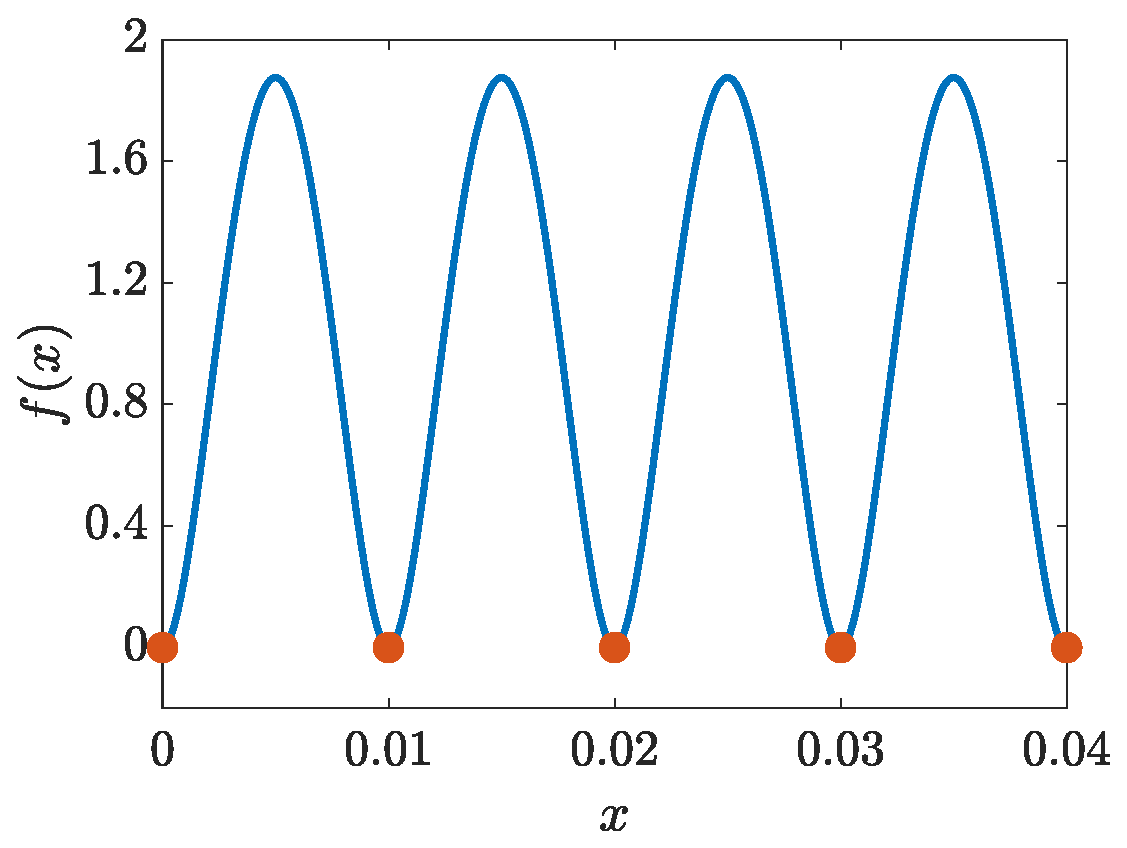
\includegraphics[width=0.3\textwidth]{ProgramsImages/SpikyFoolTrapezoidalcolor.eps} &
		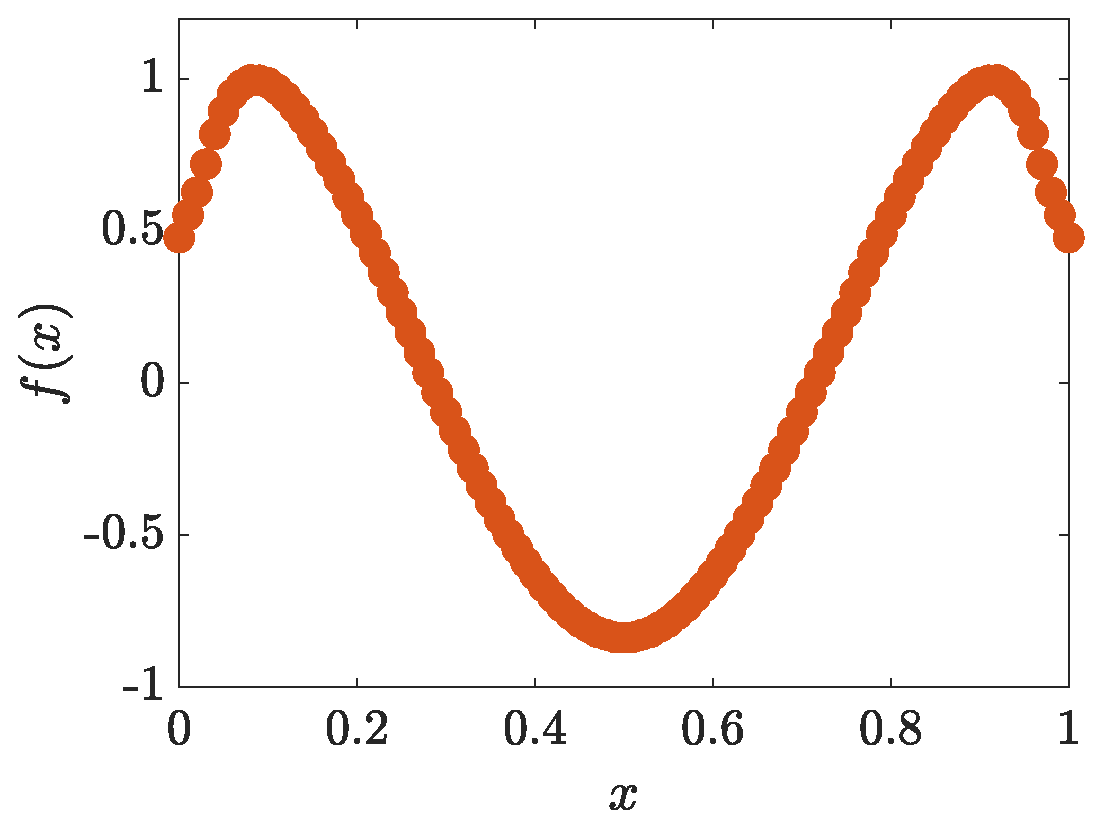
\includegraphics[width=0.3\textwidth]{ProgramsImages/FlukyFoolTrapezoidalcolor.eps} &
		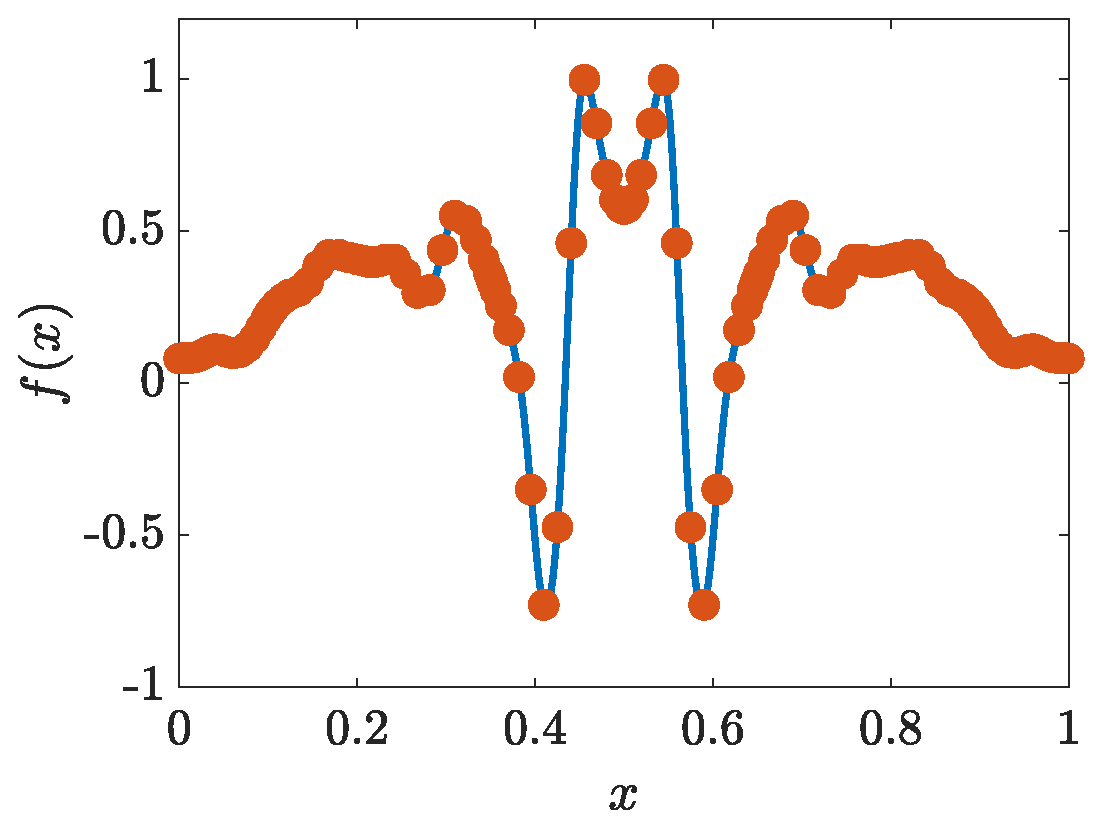
\includegraphics[width=0.3\textwidth]{ProgramsImages/FlukyFoolIntegralcolor.eps} 
		\tabularnewline
		(a) $\err_{100}(f) = 1 $ &
		(b) $\err_{100}(f) =  1.4\text{E}{-4}$ &
		(c) $\err_{150}(f) =  2.8\text{E}{-5}$
		\end{tabular}
	\caption{Integrands for which $\herr_n(f) = 0$ but 
	$\err_n(f) \ne 0$. \label{quadfail}}
\end{figure}

Despite Lyness's gloomy portrayal of adaptive quadratures, the PI and his collaborators have 
developed an adaptive trapezoidal rule that \emph{succeeds for all reasonable integrands}, although 
it 
may fail for spiky integrands \cite{HicEtal14a,HicRazYun15a}. The key is a 
data-based upper bound on $\Var(f')$.  

Here we outline the key arguments from \cite{HicRazYun15a}.  Let 
$\size(\{t_i\}_{i=0}^n) : = \max_{1 \le i \le n} t_i - t_{i-1}$ denote the partition width.  By 
definition, $\Var(f')$ is bounded below by $\widehat{V}(f',\{t_i\}_{i=0}^n)$ for any partition. 
Reasonable integrands are defined as those functions for which an inflated lower bound on  
$\Var(f')$ provides an \emph{upper bound} on $\Var(f')$:
\begin{multline} \label{conedef}
\cc := \Bigl \{ f \in C^1[0,1]: \Var(f') \le \fC(\size(\{t_i\}_{i=0}^n)) \hV(f',\{t_i\}_{i=0}^n) \text{ for all  
of }   n \in \naturals \\
 \text{and partitions } \{t_i\}_{i=0}^n \text{ with } 
\size(\{t_i\}_{i=0}^n) < \hcut \Bigr \}, \qquad  \fC(h) = \frac{\fC_0 \hcut}{\hcut - h}, \quad \fC_0 
> 1, \ 
\ 0 < \hcut < 1.
\end{multline}
This set of reasonable integrands, $\cc$, is a \emph{cone} since $f \in \cc \implies cf \in \cc$ 
for 
any 
constant $c$.  The 
parameters $\hcut$ and $\fC_0$ determine how inclusive this 
set of reasonable functions is.  It is shown in \cite{HicRazYun15a} that $\Var(f')$ can rigorously be 
bounded above by an 
inflated variation of the derivative of the linear spline, which depends only on function values, not on 
derivative values:
\begin{equation*} %\label{tVdef}
\tV_n(f) 
% & : = \sum_{i=1}^{n-1} \abs{ \frac{f((i+1)/n)-f(i/n)}{1/n} - \frac{f(i/n)-f((i-1)/n)}{1/n}}  \\& 
:= n\sum_{i=1}^{n-1} \abs{f((i+1)/n)-2f(i/n)+f((i-1)/n)}, 
\quad \Var(f') \le \fC(2/n) \tV_n(f),  \ \ 
\forall 
f \in \fC,  \ n > 2 /\hcut.
\end{equation*}
This provides a data-driven upper bound on the error  of the trapezoidal rule, namely,
\begin{equation} \label{guartraperrest}
\err_n(f) \le \oerr_n(f) \le \herr_n(f) := \frac{\fC(2/n) \tV_n(f)}{8n^2} \qquad 
\forall 
f \in \fC,  \ n > 2 \hcut.
\end{equation}
An adaptive quadrature rule is constructed by increasing $n$ until $\herr_n(f)$ does 
not exceed the error tolerance, $\varepsilon$.

\begin{algorithm}
	\caption{Adaptive Trapezoidal Rule \label{Trapalg}} 
	\begin{algorithmic}[1]
		\REQUIRE a black-box function, $f$; an absolute error tolerance,
		$\varepsilon>0$; the maximum partition width, $\hcut$; the constant $\fC_0 > 1$;  the 
		maximum number of trapezoids, $n_{\max}$

\ENSURE $\abs{\int_0^1 f(x) \dif x - T_n(f)} \le \varepsilon$, provided $f \in \cc$

\STATE $n \leftarrow \lfloor 1 /\hcut \rfloor + 1$

\REPEAT

\STATE $n \leftarrow 2n$

\STATE Compute $\herr_n(f)$ according to \eqref{guartraperrest}

\UNTIL  $\herr_n(f) \le \varepsilon$ or $n > n_{\max}$

\STATE Compute $T_n(f)$ according to \eqref{traprule}.
		
\end{algorithmic}
	\end{algorithm}


\subsection{Key Ideas Illustrated by the Adaptive Trapezoidal Rule Algorithm 
\ref{Trapalg}} 
\label{subsect:trap}

\begin{description}[leftmargin=2.5ex]
	\item[Bound the error by bounding the semi-norm of $f$] Algorithm \ref{Trapalg} succeeds 
	by 
	\emph{bounding} 
	$\Var(f')$---a key term in 
	error 
	bound \eqref{traperrbd}---for reasonable functions.  Typical  adaptive quadrature rules remain 
	flawed because they assume that the difference between two quadrature rules is indicative of the 
	error of one of them as in \eqref{tradtraperrest}.  
	
	\item[Identify a cone of reasonable functions] Our set of reasonable functions is a 
	\emph{cone} 
	defined precisely in \eqref{conedef}.  The widest spike must be wider than the minimum 
	width, $\hcut$.  
	The bound of $\Var(f')$ in terms of an inflated $ \hV(f',\{t_i\}_{i=0}^n)$ excludes large
	changes in $f'$ over small intervals.
	
	\item[The cone here is non-convex] A convex combination of two reasonable 
	functions, $f_1$ and 
	$f_2$, may produce 
	a spiky function as illustrated below (the narrow width, not the height makes it a spike):
	
	\centerline{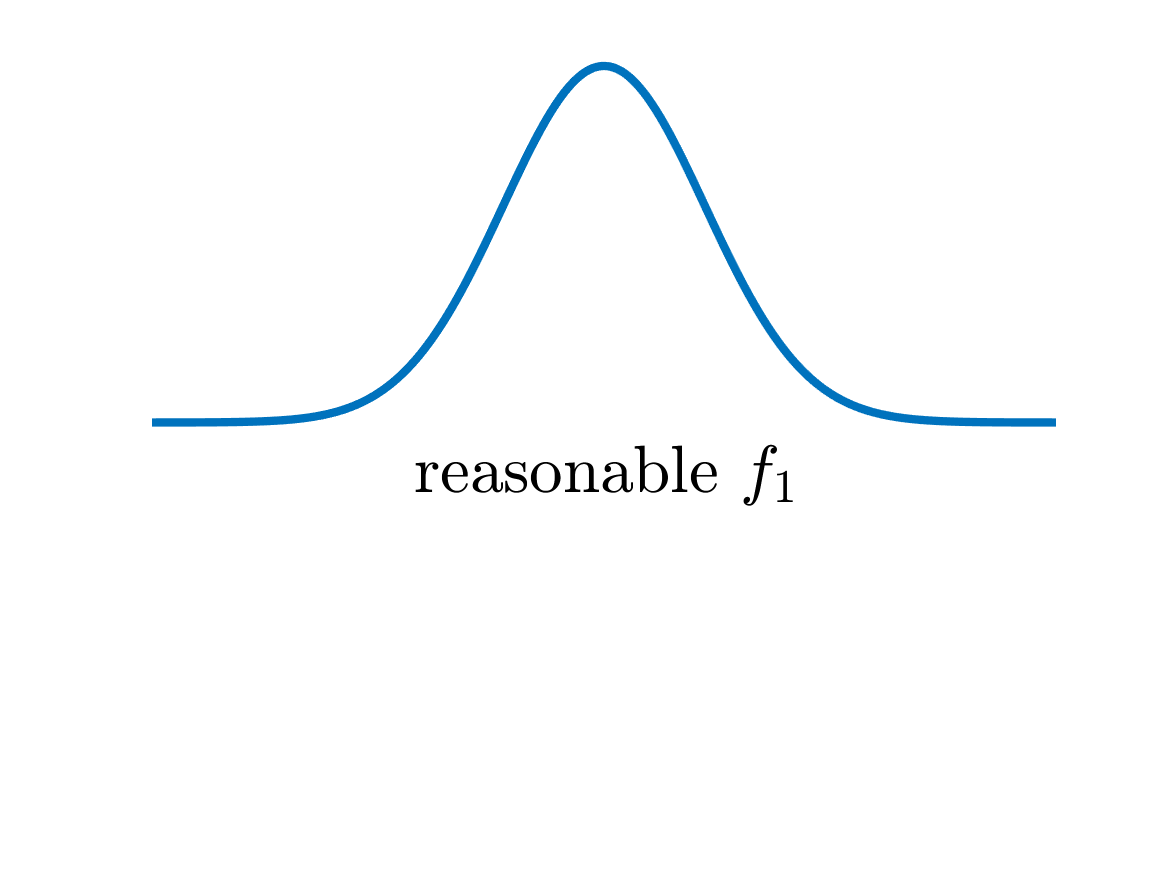
\includegraphics[width = 0.35\textwidth]{ProgramsImages/broadpk.png}
	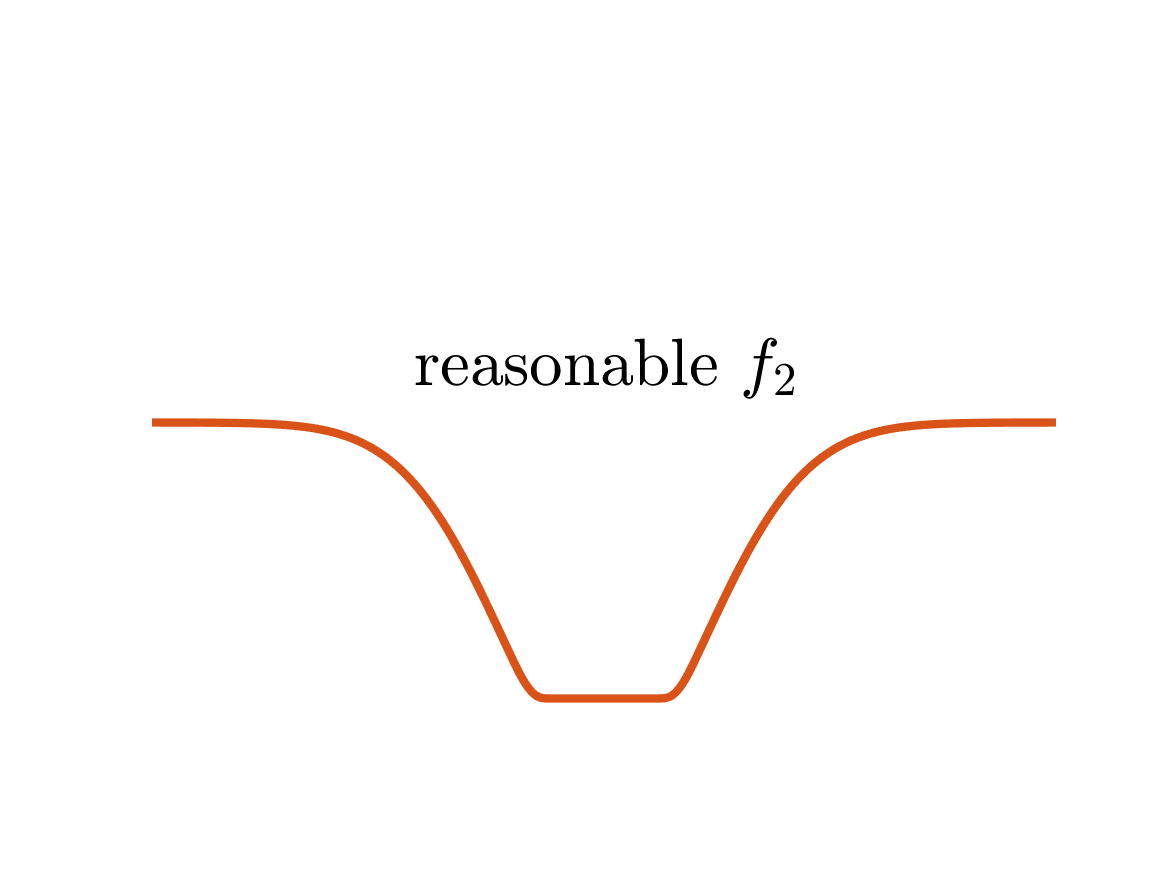
\includegraphics[width = 0.35\textwidth]{ProgramsImages/choppedpk.png}
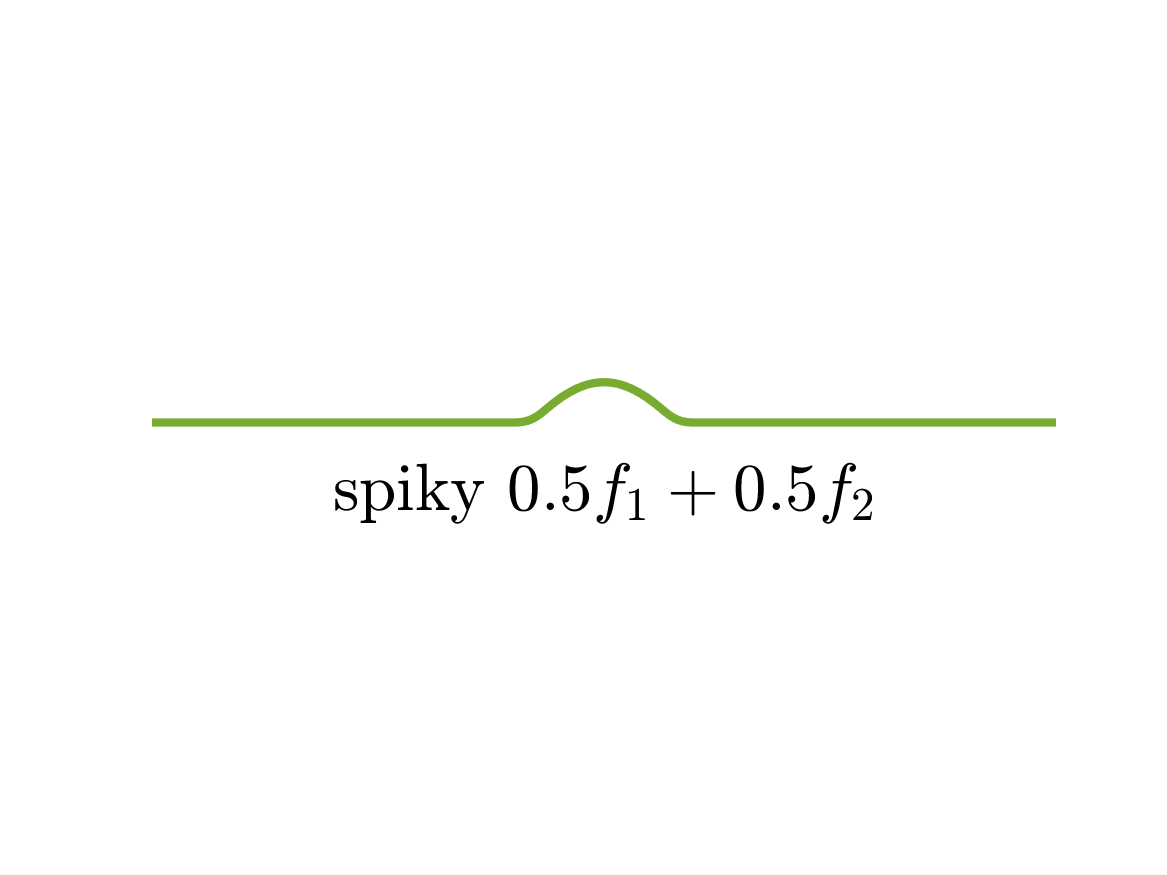
\includegraphics[width = 0.35\textwidth]{ProgramsImages/narrowpk.png}}

\vspace{-4ex}
  \noindent A non-convex cone of input functions, $\cc$, is key to an adaptive algorithm 
  that outperforms non-adaptive algorithms.  For convex sets of input functions---such as 
  balls---adaptive algorithms have no 
  advantage under rather 
  general conditions  \cite[Chap.\ 4, Corollary 5.2.1]{TraWasWoz88}.
	

	\item[Bound the computational cost of the algorithm] The number of nodes required by 
	Algorithm \ref{Trapalg} to obtain an 
	approximation 
	within an error tolerance 
	of $\varepsilon$ for $f \in \cc$ is $\Order (\Var(f')\varepsilon^{-1/2})$ \cite{HicRazYun15a}.  
	(Since $\Var(f')$ is unbounded for $f \in \cc$, we 
	include it in the expression for the computational cost.)  The computational cost for Algorithm 
	\ref{Trapalg} is asymptotically the same as that for a non-adaptive trapezoidal rule when 
	$\Var(f')$ has a known 
	upper bound.  For 
	Algorithm \ref{Trapalg} an upper bound on $\Var(f')$ is \emph{not required}.
	
	\item[Show that the adaptive algorithm is optimal] The \emph{computational complexity} of this 
	integration problem is defined as the 
	computational cost of the best 
	possible 
	algorithm to to obtain an approximation within an error tolerance 
	of $\varepsilon$ for $f \in \cc$.  It is also $\Order (\Var(f')\varepsilon^{-1/2})$ 
	\cite{HicRazYun15a}.  This 
	is 
	established by constructing fooling functions that look like zero to the algorithm, but whose 
	integral is nonzero. Thus, our algorithm is asymptotically optimal.
	
	\item[The definition of adaptive algorithm includes parameters] MATLAB's 
	\texttt{integral} \cite{MAT9.3}
	assumes an initial number of nodes and a maximum sample size.  Chebfun 
	\cite{TrefEtal17a}, a 
	numerical 
	library that adaptively integrates functions via Chebyshev polynomial approximations 
	assumes 
	default values for these parameters as well as others.
	These parameters are set to be reasonable for most situations, but may be modified if 
	necessary.  The parameters  $\hcut = 0.02, \fC_0 = 
	1.5$, and 
	$n_{\max} = 10^7$ are meant to remain the same from problem to problem, but may be 
	modified 
	to 
	enhance speed or increase robustness.
	
	\item[The adaptive algorithm is available]  Algorithm 1 and related adaptive algorithms 
	developed 
	by the PI and his collaborators have been published in the Guaranteed Automatic 
	Integration 
	Library (GAIL) \cite{ChoEtal17b}.  We propose to further develop this library (Section 
	\ref{}).
	
	\item[Error bound exists even if  time is the limiting factor]  Specifying the number of 
nodes rather than the error tolerance is accomplished by setting $n_{\max}$ to be this
 number and $\varepsilon = 0$.  The error bound, $\herr_n(f)$, is not needed to 
stop the algorithm but is available to inform the user how large the error might be.

	\item[Adaptivity here is only for the number of nodes] While the  quadrature algorithm 
	described 
	above is 
	adaptive in determining the $n$ (gloabal adaptivity), it is not adaptive in determining the 
	placement of the nodes (local adaptivity).  
	However, Section 
	\ref{previousmeritsubsec} below describes work in that direction for function 
	approximation and optimization.
	
	\item[Optimality is only for integrands with limited smoothness] This adaptive quadrature rule is 
	optimal for the cone of integrands, $\cc$, however, it is 
	sub-optimal for smoother integrands.  See Section \ref{?} for proposed research in this direction.
	
\end{description}

Our proposed research addresses a class of problems beyond univariate integration.  The next two 
subsections provide the notation for these problems and outline our research goals.


\subsection{Traditional Error Analysis} Let $\calf$ be a Banach space of input functions 
defined on the domain $\cx$, let
$\calg$ be a Banach space of possible 
solutions, and let $S:\calf \to \calg$ be a solution operator.  Ignoring for now the precise definitions 
of $\calf$ and $\calg$, some examples of solution 
operators for integration, function approximation (recovery), and optimization are
\begin{equation} \label{probs}
S = \INT: f \mapsto \int_{\Omega} f(\bx) \, \dif \bx, \qquad S = \APP:f \mapsto f, \qquad S = 
\OPT :f \mapsto 
\min_{\bx \in \Omega} f(\bx).
% \\S: f \mapsto u, \text{ where } u'' + u = f(x), \quad u(0) = u(1) = 0.
\end{equation}
Let $\{A_n: 
\calf \to \calg\}_{n \in \calI}$ be a sequence of algorithms.  Each $A_n$  samples the 
input function, 
$f$, at $n$ nodes
(data sites) $\desn \subset \cx$, and produces an approximation to $S(f)$ based 
on $\{(\bx_i,f(\bx_i))\}_{i=1}^n$.
Here 
$\calI$ is an index set of positive integers. 

The error bounds  for $A_n$ typically take the  form
\begin{gather} \label{typicalerr}
\err_n(f): = \norm[\calg]{S(f) - A_n(f)} \le \norm{A_n} \norm[\calf]{f} =: \oerr_n(f) \qquad \forall f \in 
\calf, \ n \in 
\calI, 
\\ \text{where }\norm{A_n}  : = \sup_{0 \ne f \in \calf} \frac{\norm[\calg]{S(f) - A_n(f)}} 
{\norm[\calf]{f}}.
\end{gather} 
In some cases, such as  \eqref{traperrbd}, $\norm[\calf]{f}$ is a 
semi-norm rather than a norm.  The term $\norm{A_n}$
represents the worst case error for functions in the unit ball in $\calf$ and is a quality measure for 
the algorithm, including the
choice of nodes.  In some cases 
$\norm{A_n}$ has an explicit expression ($1/(8n^2)$ in \eqref{traperrbd}), whereas in other 
cases one 
can only derive an upper bound on $\norm{A_n}$ or the convergence rate of 
$\norm{A_n}$. 
Error bounds of the form  \eqref{typicalerr} are typically 
illustrated by plotting $\norm[\calg]{S(f) - A_n(f)}$ versus $n$ for some example $f$ and showing 
that the 
convergence rate has the same order as $\norm{A_n}$.

\subsection{Adaptive Algorithms} A practical problem is choosing  $n$ to satisfy an 
error criterion, e.g.,
\begin{equation} \label{errorcrit}
\norm[\calg]{S(f) - A_n(f)} \le \varepsilon \quad \text{where the tolerance } \varepsilon 
\text{ is 
specified by the user}.
\end{equation}
Theoretically, the best choice is $n = \min \{ n' \in \calI : \norm{A_n} \le \varepsilon / 
\norm[\calf]{f}\}$.  However, even if $\norm{A_n}$ is known explicitly, $\norm[\calf]{f}$ is 
typically 
unknown and cannot be 
bounded easily.  Thus, the error bound $\oerr_n(f)$ in \eqref{typicalerr} does not directly lead to
a  data-based
criterion for adaptively choosing $n$.  

Adaptive algorithms rely on error bounds, $\herr_n(f)$, computed from function data, 
$\{(\bx_i,f(\bx_i))\}_{i=1}^n$, and not a priori knowledge of the (semi-)norm of the function.  Those 
commonly used in practice are inadequate because there is no theoretical justification that 
$\oerr_n(f)  \le \herr_n(f)$.  As mentioned earlier MATLAB's \texttt{integral} bases its $\herr_n(f)$ on 
the comparison of two Gaussian quadratures.  Chebfun determines the number of polynomials 
required to approximate a function approximation of functions by Chebyshev polynomials by 
determining when the coefficients of the higher degree polynomials have reached round-off 
error.

There is a family of adaptive integrals with a theoretical foundation based on interval 
arithmetic 
described in \cite{MoKeCl09} and \cite{Rum10a} and implemented in INTLAB \cite{Rum99a}.  
This 
approach requires the function subroutines to take interval arguments and return interval 
outputs.  
We are not following this approach because existing black-box, user-defined subroutines 
normally 
do not meet these requirements, and for multidimensional problems, which are of particular 
interest, 
interval arithmetic may be quite slow.

For Algorithm \ref{Trapalg}  of Section \ref{subsect:trap}, $\norm[\calf]{f}$ is bounded in 
terms of function data for reasonable functions in a cone, $\cc \subset \calf$. This allows us 
to 
construct an adaptive quadrature rule that has a theoretical foundation and that is 
asymptotically the best possible algorithm for 
approximating the solution to within the given error tolerance.  


\subsection{What Comes Next}
Our numerical algorithm for computing $\cos(x)$ to the desired accuracy---typically machine 
precision---does not require the user to determine how many terms in the polynomial 
approximation are required.  The computation is automatic.  Furthermore, there is theory 
that justifies this algorithm.  

We believe that the same should be possible for somewhat more complex problems, such as 
those in \eqref{probs}.
Our recent NSF-Funded research---summarized in the next section---has developed 
some such adaptive numerical algorithms based on the ideas illustrated in Section 
\ref{subsect:trap}.  These adaptive algorithms that have theoretical basis in that they are 
proven to work for input functions in clearly defined cones, $\cc$; the stopping criteria are 
not heuristics. These algorithms have been implemented in GAIL \cite{ChoEtal17b}, and their 
effectiveness has been demonstrated on various practical problems.  The research proposed 
in Section \ref{secProposed} aims to significantly enlarge the family of adaptive numerical 
algorithms that have both a theoretical basis and practical application.

\section{Results of Previous NSF-Funded Research,
NSF-DMS-1522687\except{toc}{, \emph{Stable, Efficient, Adaptive Algorithms for 
Approximation and 
Integration}, 
\$270,000, 2015--2018}} \label{SectPrevious}

G. E. Fasshauer (GEF, co-PI) and F. J. Hickernell (PI) have led this project.  In the summer of 
2016, Fasshauer left Illinois Tech and has participated since then as a sub-contractor.  
Sou-Cheng Choi (SCC) has contributed as a senior personnel.  Other major contributors 
have been the PI's research students Yuhan Ding (YD, PhD 2015), Lan Jiang (LJ, PhD 2016), 
Llu\'is Antoni Jim\'enez Rugama, Da Li (DL, MS 2016), Jagadees Rathinavel (JR, PhD student)
Xin Tong (XT, MS 2014, PhD student, University of Illinois at Chicago), Kan Zhang (KZ, PhD 
student), Xuan Zhou (XZ, PhD 2015)


\subsection{Intellectual Merit from Previous NSF Funding}
\label{previousmeritsubsec}

\subsubsection{Local Adaption for Univariate Problems} The PI, SC, YD, and XT developed 
locally adaptive 
algorithms for univariate function 
approximation and 
global optimization \cite{ChoEtal17a}, i.e., cases $\APP$ and $\OPT$ in 
\eqref{probs} for $\Omega = [a,b]$.  
The error of the \emph{linear spline}, $A_n$, using the 
nodes $a = x_0 < x_1 < \cdots < x_n = b$,  in approximating a function is 
\begin{equation} \label{linsplineerror}
\norm[{\infty,[x_{i-1},x_i]}]{f - 
	A_n(f)} \le \frac{(x_i-x_{i-1})^2\norm[\infty,{[x_{i-1},x_i]}]{f''}}{8} =: \oerr_n(f,[x_{i-1},x_i]),
\end{equation}
where $\norm[{\infty,[\alpha,\beta]}]{\cdot}$ denotes the sup-norm over the interval 
$[\alpha,\beta]$.  The cone of reasonable functions, $\cc$, consists essentially of those 
functions for 
which the local supremum of $f''$ is bounded above by an inflated value of the local infimum 
of $f''$ to the left or the right (see \cite{ChoEtal17a} for details):
\[
\cc: = \left \{ f \in W^{2,\infty} : \norm[{\infty,[\alpha,\beta]}]{f''} \le \max\left(\fC(h_{-}) 
\norm[-\infty,{[\beta-h_-,\alpha]}]{f''},\fC(h_{+})
\norm[-\infty,{[\beta, \alpha+h_+]}]{f''}\right) \  \forall h_{\pm} \le \hcut \right\},
\]
where $\fC(\cdot)$ is the inflation factor in \eqref{conedef}, and $\norm[-\infty,{[\alpha, 
\beta]}]{f''} = \inf_{\alpha \le x \le \beta} \abs{f''(x)}$.  Because one looks at the infimum of the 
second derivative on both sides, 
a reasonable function may have inflection points, but two inflection points may not be too 
close together.  

For 
reasonable functions, there exists a data-based error bound 
$\herr_n(f,[x_{i-1},x_i]) \ge \oerr_n(f,[x_{i-1},x_i])$ defined in terms of second order 
difference 
quotients on the 
left and right sides of $[x_{i-1},x_i]$.  Each interval $[x_{i-1},x_i]$ is refined until  
$\herr_n(f,[x_{i-1},x_i]) \le \varepsilon$.  The resulting linear spline, $A_n(f)$, satisfies error 
criterion \eqref{errorcrit} for the function approximation problem. Figure 
\ref{localadaptfig} (left) displays an example of the function data required.  The function is 
sampled sparsely where the second derivative is small.

\begin{figure}
	\centering
	\vspace{-12ex}
	\includegraphics[width = 0.48\textwidth]{ProgramsImages/sampling-funappxg.png}
	\includegraphics[width = 0.48\textwidth]{ProgramsImages/sampling-funming.png}
	
	\vspace{-12ex}
	\caption{The function data ({\color{MATLABOrange}$\bullet$}) for  locally adaptive 
	function approximation  (left) and locally adaptive optimization (right) \label{localadaptfig}}
\end{figure}


The computational cost of this locally adaptive approximation algorithm is 
$\Order\left(\sqrt{\norm[1/2]{f''}/\varepsilon} \right)$ \cite{ChoEtal17a}, where 
$\norm[1/2]{\cdot}$ is the $1/2$-quasinorm, which is weaker than the sup-norm.  This is  
asymptotically the same cost as for the best possible algorithm for this problem. In contrast, 
the globally adaptive function approximation algorithm in \cite{HicEtal14b} has a 
computational cost of $\Order\left(\sqrt{\norm[\infty]{f''}/\varepsilon} \right)$.  For a spiky 
function inside $\cc$, the local adaption algorithm may require significantly less effort 
than a global adaption algorithm because $\norm[1/2]{f''}$ will be much smaller than 
$\norm[\infty]{f''}$.

Similar arguments to those above lead to a locally adaptive algorithm for the 
optimization problem, $\OPT$ in \eqref{probs}.  In this case, those subintervals for which the 
function is definitely greater than the minimum found so far need not be 
refined further.  Figure 
\ref{localadaptfig} (right) gives an example of the function data required.  The function is 
sampled sparsely where the second derivative is small or the function is large.

\subsubsection{Global Adaption for Multidemsional Integration}

e only 
intervals that require refinement are those which might contain minimum

Project 1. 
a) Fasshauer collaborated with Jalil Rashidinia and Manoochehr Khasi on an alternative 
approach to implementing Hilbert-Schmidt eigenfunctions of the Gaussian kernel by using 
Chebyshev polynomials instead of Hermite polynomials in the expansion used in our earlier 
work. This enhances the numerical stability of the algorithm. This new eigenfunction 
representation was also applied to the numerical solution of nonlinear unsteady 
convection-diffusion-reaction equations.

b) Fasshauer has been collaborating with Paul Martin to extend an earlier derivation for 
eigenfunctions and eigenvalues of the $C^0$ Matern kernel on the half line from the 
monograph Fasshauer and McCourt (2015) to the entire real line. Extensions to smoother 
Matern kernels are currently being investigated. 

Project 1. 
a) A paper has been submitted that details the new Chebyshev polynomial-based 
eigenfunction representation of the Gaussian kernel and uses this representation to solve 
nonlinear unsteady convection-diffusion-reaction equations.

b) So far, we have been able to extend earlier results for low-order Matern kernels from the 
half-line to the entire real line. We are looking for ways to "lift" the techniques to accomplish 
this to the case of higher-order Matern kernels before preparing a paper on the topic.


To our knowledge, it is the first time that eigenfunctions and eigenvalues on the real line for 
a kernel in the Matern family have been derived analytically. Thus far, such results were 
available only on bounded intervals.   





partially supported 
\cite{ChoEtal17a,GilEtal16a,HicEtal17a,HicJim16a,JimHic16a,ZhoHic15a,ChoEtal17b,HicEtal18a}.



\subsection{Broader Impacts from Previous NSF Funding}

Project 1. 
a) Fasshauer collaborated with Jalil Rashidinia and Manoochehr Khasi on an alternative 
approach to implementing Hilbert-Schmidt eigenfunctions of the Gaussian kernel by using 
Chebyshev polynomials instead of Hermite polynomials in the expansion used in our earlier 
work. This enhances the numerical stability of the algorithm. This new eigenfunction 
representation was also applied to the numerical solution of nonlinear unsteady 
convection-diffusion-reaction equations.
Project 1. 
a) Fasshauer collaborated with Jalil Rashidinia and Manoochehr Khasi on an alternative 
approach to implementing Hilbert-Schmidt eigenfunctions of the Gaussian kernel by using 
Chebyshev polynomials instead of Hermite polynomials in the expansion used in our earlier 
work. This enhances the numerical stability of the algorithm. This new eigenfunction 
representation was also applied to the numerical solution of nonlinear unsteady 
convection-diffusion-reaction equations.
Project 1. 
a) Fasshauer collaborated with Jalil Rashidinia and Manoochehr Khasi on an alternative 
approach to implementing Hilbert-Schmidt eigenfunctions of the Gaussian kernel by using 
Chebyshev polynomials instead of Hermite polynomials in the expansion used in our earlier 
work. This enhances the numerical stability of the algorithm. This new eigenfunction 
representation was also applied to the numerical solution of nonlinear unsteady 
convection-diffusion-reaction equations.




\section{Intelletual Merit of Proposed Research} \label{secProposed}


\section*{Research Project 1. Extensions of the Hilbert--Schmidt SVD}\label{SectHSSVD}



\section*{Research Project 2. Extensions of Guaranteed, Adaptive Algorithms}\label{SectGAIL}

doit Roshan

\begin{figure}[htbp]
\centering
\begin{tabular}{>{\centering}m{6cm}@{\hspace{1cm}}>{\centering}m{6cm}}
\includegraphics[width=6cm]{SpikyFoolIntegral.pdf} \newline
 $\int_0^1 f_{\text{spiky}}(x) \, \dif x=0.5$
 &
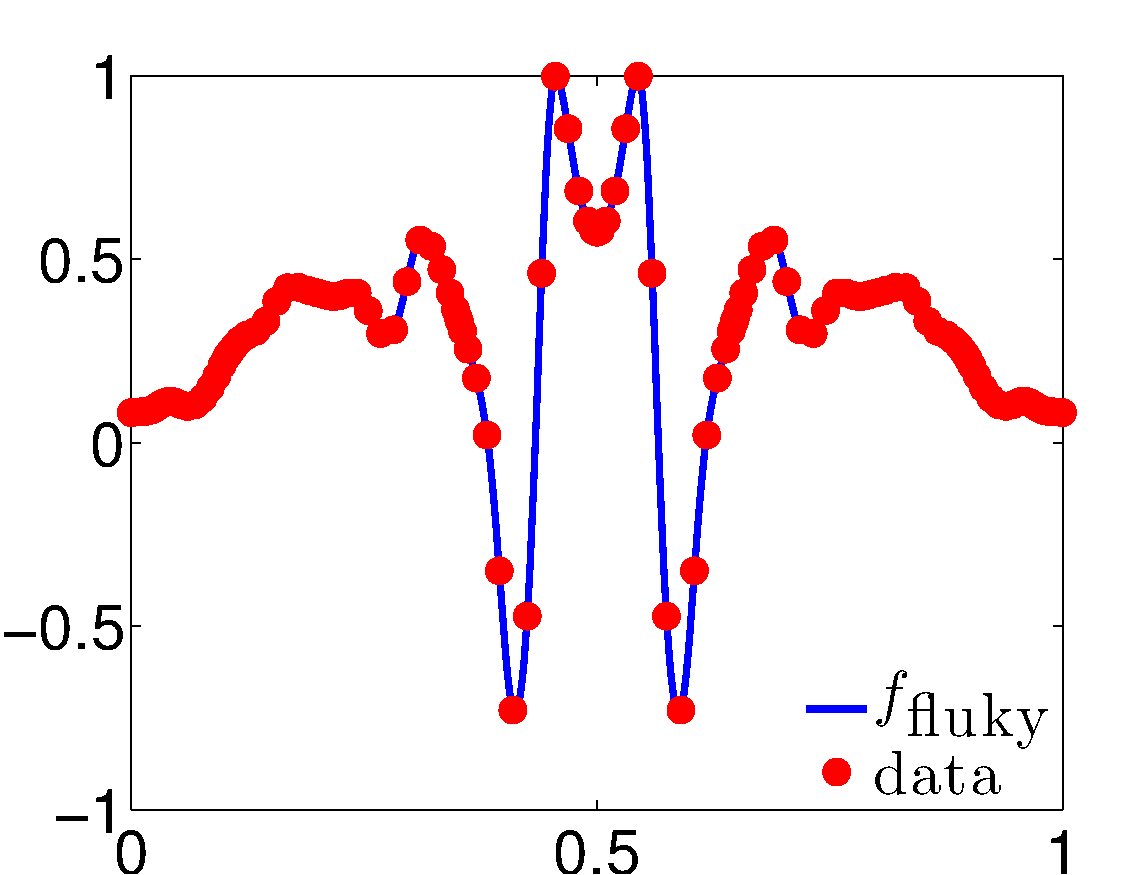
\includegraphics[width=6cm]{FlukyFoolIntegral.pdf} \newline
 $\int_0^1 f_{\text{fluky}}(x) \, \dif x=0.278827$
\end{tabular}
\texttt{integral(fspiky,0,1,'AbsTol',1e-13,'RelTol',1e-13)={\color{red}0}} \\
\texttt{integral(ffluky,0,1,'AbsTol',1e-13,'RelTol',1e-13)=0.278{\color{red}799}}
\caption{Integrands for which \Matlab's {\tt integral} fails to give the answer to within the user-specified tolerance. \label{MatIntegFailFig}}
\end{figure}

\Matlab has no adaptive (quasi-)Monte Carlo cubature methods (guaranteed or not).  The Chebfun \Matlab toolbox \citep{TrefEtal14} solves a host of problems adaptively, but has no theoretical guarantees.  Our proposed new adaptive algorithms will build upon our previous work and provide guarantees of success, upper bounds on computational cost, and proof of asymptotic optimality.

As a side note, we are aware of the extensive literature on guaranteed algorithms via \emph{interval arithmetic}. This approach, is described in \cite{MoKeCl09} and \cite{Rum10a} and implemented in INTLAB \cite{Rum99a}.  We are not pursuing this approach, because we do not want to require our functions to provide interval outputs, and we think that this approach has limitations, especially for larger dimensions.

\subsection*{Research Project 2.1. Adaptive (Quasi-) Monte Carlo Algorithms for Multivariate Integration}\label{Integrationsubsec}
Multivariate integrals may be approximated by averaging function values:
\begin{equation} \label{integprob}
I(f) := \int_{\reals^d} f(\bx)  \, \varrho(\bx) \, \dif \bx \approx
\frac 1 N \sum_{i=1}^N f(\bx_i) =: \hI_N(f).
\end{equation}
Here $\varrho$ is a probability density function, and the well-chosen data sites come from an infinite sequence $\desinf$, which allows $N$ to be chosen adaptively.  We have in mind situations where $f$ is insufficiently smooth or $d$ is too large for tensor product rules to be competitive.  Two popular choices are (i) independent and identically distributed (IID) points with density $\varrho$---simple Monte Carlo sampling---and (ii) suitably transformed low discrepancy sequences, such as digital or integration lattice sequences---quasi-Monte Carlo sampling \citep{DicPil10a,DicEtal14a,Lem09a,Nie92,Owe13a,SloJoe94}.

We have already constructed a simple Monte Carlo algorithm \citep{HicEtal14b} and two quasi-Monte Carlo algorithms \citep{HicJim16a,JimHic16a}, that \emph{adaptively} choose the sample size, $N$, in a way that rigorously ensures that the user-specified error tolerance is satisfied:
\begin{equation} \label{cubMCguar}
\bigabs{I(f) -\hI_N(f)} \le \abstol \quad \text{or} \quad \Prob\bigl[\bigabs{I(f) -\hI_N(f)} \le \abstol \bigr] \le 1-\alpha,
\end{equation}
the former holding for deterministic quasi-Monte Carlo sampling, and the latter holding for simple Monte Carlo sampling and confidence level $1-\alpha$.  All three adaptive algorithms base their decisions on data-driven error estimates, rather than a priori knowledge of the integrands.

We will extend these algorithms to handle a hybrid absolute/relative error tolerance of the form $\max(\abstol,\reltol \abs{I(f)})$, which is more flexible than our present pure absolute error tolerance, $\abstol$.  Since we already know how to estimate the error from the data, this problem is partially solved.  The missing piece is how to estimate $I(f)$ appearing in the error tolerance, $\max(\abstol,\reltol \abs{I(f)})$.  This will require an unspecified number of iterations.  For the simple Monte Carlo algorithm we must ensure that all these iterations combined stay within the specified confidence level.

We also propose to add control variates to our adaptive (quasi-)Monte Carlo algorithms.  Given an integrand $g$ whose integral, $I(g)$, is known, the control variate estimator is $\starred{I}_{N}=\hI_N(f) + \beta [ I(g) - \hI_N(g)]$.  For simple Monte Carlo sampling there is a standard way to estimate the optimal $\beta$, but this method may give the wrong answer for low discrepancy sampling \citep{HicEtal03}.  We will use the insight in \citep{HicEtal03} to find a better way of determining $\beta$ for low discrepancy sampling.

Option pricing is an important application of multivariate integration.  When the stock price is monitored continuously we have the  limiting case of $d\to \infty$.  Multi-level methods \citep{Gil14a,Hei01a,HicMGRitNiu09a,NiuHic09b} have been found to be successful in efficiently evaluating infinite dimensional integrals.  We will extend our existing adaptive (quasi-)Monte Carlo algorithms to become adaptive multi-level methods for $d \to \infty$.  The unbiased approach of \cite{RheGly12a} looks very promising.

Besides establishing rigorous guarantees for our new algorithms, we also will establish upper bounds on the computational cost of these algorithms.  As in our previous work, the cost will depend on the known input parameters, such as the error tolerance(s) and the uncertainty, $\alpha$, as well as on unknown quantities, such as the variance of $f(\bX)$, $\bX \sim \varrho$ (for simple Monte Carlo) and the rate of decay of the series coefficients for $f$ (for quasi-Monte Carlo).  We also propose to show that these computational costs are asymptotically optimal relative to the best possible algorithms that make the same assumptions on the set of possible integrands.  This will be done by using bump functions, a well-known method in the information-based complexity literature (see \cite{Nov88,TraWasWoz88}).

\subsection*{Research Project 2.2. Higher Order and Locally Adaptive Univariate Function Approximation and Integration}\label{Higherordersubsec}
In our previous NSF-funded project (see Sect.\ \ref{previousmeritsubsec}) we developed adaptive univariate function approximation and integration algorithms based on linear splines, but \emph{with rigorous guarantees of success} \citep{HicEtal14b}.  In our proposed work we will extend these methods in two directions.  One obvious goal is to increase the efficiency by using higher order function approximation than the linear spline. The general framework provided in \cite{HicEtal14b} will facilitate this.

All of our adaptive algorithms for univariate or multivariate problems developed so far have been globally adaptive, i.e., the design, $\desinf$, is fixed but the number of data, $N$, is determined adaptively.  A second goal of this project  is to introduce local adaption, i.e., algorithms where the density of the data sites, as well as their number, depends on the function data.  This is easiest to do for univariate problems---in fact, it is done by others now, but without theoretical guarantees.  We will sub-divide the whole function domain (an interval) into sub-intervals and solve function approximation or integration problems separately on those.  These subdivisions will be data driven.

Finally, as was done for the original algorithms in \citep{HicEtal14b}, we will derive upper bounds on the costs of our new higher order and locally adaptive algorithms.  We will also demonstrate their asymptotic optimality by using bump functions \cite{Nov88,TraWasWoz88}.

\subsection*{Why Cones} The adaptive algorithms that we have derived in our previous work, and the adaptive algorithms that we propose to derive are or will be \emph{guaranteed} to satisfy the user-specified error tolerance.  This sets them apart from existing adaptive algorithms, which have no such guarantees.

Obtaining rigorous guarantees of success for adaptive algorithms requires limiting the functions to some set, $\calc$.  Our experience and expectation is that $\calc$ turns out to be a \emph{cone} of functions.

There are good reasons for this. The true absolute error of function approximation, $\err(f,N):=\bignorm[\infty]{f-\tf}$, or integration, $\err(f,N):= \bigabs{I(f) - \hI_N(f)}$, is positively homogeneous, i.e., $\err(cf,N)=\abs{c} \err(f,N)$. We also expect any reasonable data-driven error bound, $\oerr(f,N)$, to also be positively homogeneous.  Thus, the set of functions for which the error bound is correct, $\calc:=\{f : \err(f,N) \le \oerr(f,N)\}$, must be a cone, since $f\in \calc \implies cf \in \calc$.

%The traditional error analysis works with \emph{balls} of input functions, $\cb :=\{ f : \norm[\ch]{f} \le \sigma\}$, where $\ch$ is some normed vector space of functions, and $\sigma$ is the radius of the ball.  For example, see (\ref{powfunerrbd}, \ref{filldiserrbd}) below.  Unfortunately, an algorithm that works for $f \in \cb$ may fail for $c f$ if $c>1$.

Moreover, it is known that adaptive algorithms cannot outperform non-adaptive algorithms for functions in convex sets, such as balls \cite[Chapter 4, Theorem 5.2.1]{TraWasWoz88}. Because cones need not be convex (think of a hollow ice cream cone), adaptive algorithms may be advantageous for cones of input functions.

\section*{Research Project 3. Constructing Guaranteed, Adaptive Kernel Methods} \label{combinesec}

\subsection*{Research Project 3.1. Data-Driven Error Estimation}\label{errestsubsec} Our goal is to construct adaptive multivariate function approximation algorithms using kernel algorithms of the form \eqref{rbfapprox}, but perhaps using the Hilbert--Schmidt SVD for stable computation.  This requires an error bound, $\oerr(f,N)$, based on the function data, that conservatively estimates the true error, $\err(f,N):=\bignorm[\infty]{f-\tf}$. Cross-validation (CV) is sometimes used to approximate the error. One form of CV is
\begin{subequations} \label{rbferrbd}
\begin{multline} \label{crossvalid}
\err(f,N) \\
\approx \sqrt{\frac{C}{N} \left[ \sum_{i=1}^{N/2} \abs{f(\bx_{2i-1})-\tf(\bx_{2i-1};\{\bx_{2i}\}_{i=1}^{N/2})}^2 + \sum_{i=1}^{N/2} \abs{f(\bx_{2i})-\tf(\bx_{2i};\{\bx_{2i-1}\}_{i=1}^{N/2})}^2 \right]}.
\end{multline}
Using the same notation as in \refproba, there also exist rigorous error bounds for functions in the Hilbert space $\ch_K$ with reproducing kernel $K$ of the form \citep{Wen05a}
\begin{align}
\label{powfunerrbd}
\err(f,N) & \le \sqrt{\sup_{\bx \in \cx}[K(\bx,\bx)-\bk(\bx)^T\mK^{-1} \bk(\bx)]} \norm[\ch_K]{f} \\
\label{filldiserrbd}
\err(f,N) & \le C [\filldis(\desn)]^r \norm[\ch_K]{f}, \qquad
\filldis(\desn): = \sup_{\bx \in \cx} \min_{i=1,  \ldots, N} \norm[2]{\bx - \bx_i}.
\end{align}
\end{subequations}

All of these expressions have drawbacks as candidates for a data-driven $\oerr(f,N)$.  CV has no finite-sample size guarantees of successfully providing an upper bound on the true error.  The error bounds in (\ref{powfunerrbd}, \ref{filldiserrbd}) require $\norm[\ch_K]{f}$, which is not known a priori. Computation of $\bk(\bx)^T\mK^{-1} \bk(\bx)$ may suffer from stability issues.  Taking the supremums in (\ref{powfunerrbd}, \ref{filldiserrbd}) is nontrivial. While $r$ denotes the kernel smoothness in \eqref{filldiserrbd}, the constant $C$ is not always known explicitly.

We propose finding guaranteed data-driven error bounds for functions in certain  \emph{cones}.  Given our experience with the integration problem, these cones may take the form of a strong norm of $f$ being bounded above by a weaker norm of $f$, as in \cite{HicEtal14b}, which rules out spiky functions.  This may allow us to rigorously justify the CV. Alternatively, our cones may involve assumptions on the decay rates of the series representations of the functions in terms of the basis, $\{\varphi_n\}_{n=1}^{\infty}$, as in \cite{HicJim16a,JimHic16a} and suggest that we calculate directly with a well-chosen, stable, data-dependent basis---rather than the kernel---as in \refproba.  We may find some other way to overcome the drawbacks for one of the error bounds listed above.  For example, the results of \refproba may help us overcome the instability associated with expressions involving $\mK^{-1}$.

%The Hilbert--Schmidt series of the iterated Brownian bridge kernels \citep{CavorettoEtAl14} is given by
%\begin{equation}\label{IBBkernel}
%K(x,t) = \sum_{n=1}^{\infty} \left(n^2\pi^2 + \gamma^2\right)^{-\beta} 2\sin(n\pi x) \sin(n\pi t), \quad x,t \in [0,1],\ \gamma>0, \beta \in \mathbb{N},
%\end{equation}
%and therefore it is a perfect candidate for the data-driven error bounds discussed above since the eigenfunctions do not depend on the parameters $\beta$ and $\gamma$, while a smaller smoothness parameter $\beta$ leads to slower decay of the eigenvalues.

The Hilbert--Schmidt series of a family of kernels generalizing the periodic spline kernels of \citep[Chapt.~2]{Wah90} is given by
\begin{align}\label{PeriodicKernel}
K(x,t) &= \sum_{n=1}^\infty \left(4n^2\pi^2 + \gamma^2\right)^{-r/2} 2\left(\cos (2n\pi x) \cos (2n\pi t) + \sin (2n\pi x) \sin (2n\pi t)\right) \\
 &= \sum_{n=1}^\infty \left(4n^2\pi^2 + \gamma^2\right)^{-r/2} 2\cos\left(2n\pi(x-t)\right), \quad x,t \in [0,1],\ \gamma>0, r \in \mathbb{N}. \nonumber
\end{align}
This is a perfect candidate for the data-driven error bounds discussed above since the eigenfunctions do not depend on the parameters $r$ and $\gamma$, while a smaller smoothness parameter $r$ leads to slower decay of the eigenvalues.


\subsection*{Research Project 3.2. Data-Driven Parameter Estimation} \label{parestsubsec}
Parameters of the kernel $K$---such as the shape parameters $\gamma_\ell>0$ for the anisotropic Gaussian kernel in \eqref{gausskernel}, or the smoothness and shape parameters, $r$ and $\gamma$, for the Mat\'ern kernels in \eqref{Maternkernels}---may be determined by maximum likelihood estimation (MLE).  In practice, one usually assumes that underlying function is one instance of a Gaussian stochastic process, and then one uses the profile log-likelihood $\ell(\bgamma) = N\log(\by^T\mK^{-1}\by) + \log(\det(\mK))$ to estimate the ``best'' kernel parameters. Here these parameters are collected in the vector $\bgamma$.  The sample size, $N$, and the vector of given function values, $\by$, are as in \eqref{rbfcoef}. Since the matrix $\mK$, which depends on $\bgamma$, can easily become \emph{ill-conditioned even for moderate $N$} the profile log-likelihood needs to be computed with a stable numerical algorithm such as the Hilbert--Schmidt SVD since it becomes unreliable otherwise (see Fig.~\ref{Fig_HSSVD}).
%The ill-conditioning will arise if the kernel has a high degree of smoothness, and/or if it becomes ``flat'' (the $\gamma_\ell$ are near zero). This means that $f$ is very smooth and the discretization error \eqref{rbferrbd} vanishes rapidly as the fill distance decreases.
As Fig.~\ref{Fig_HSSVD} also shows, for any given set of data, finding an ``optimal'' (or near-optimal) value of the kernel parameter(s) can have a significant impact on the accuracy of the recovered function $\tf$. A number of potential criteria for optimizing kernel parameters were introduced in \citep{Fasshauer11}. However, up to now all of those criteria were based on the use of the standard approach, i.e., they were subject to the effects of ill-conditioning of $\mK$, and thus often unreliable or impractical. Recently, the MLE criterion (or more precisely, profile log-likelihood) was the first of these criteria to be converted to the stable framework \citep{McCourtFas14}, and this is the approach used in the right part of Fig.~\ref{Fig_HSSVD}. We propose to extend the application of the Hilbert--Schmidt SVD to other criteria, and then to investigate which of these criteria is most effective.


\subsection*{Research Project 3.3. Data-Driven Designs} \label{designsubsec}
An important issue is not only the surface fitting problem itself, but also the choice of \emph{design}, i.e., the data locations or choice of inputs $\bx_i$. The main objectives for finding a ``good'' design are that it successfully deal with the \emph{curse of dimensionality}, i.e., that it effectively fill out the high-dimensional design space, and that it ensure an accurate solution of the scattered data fitting problem. In many realistic surrogate modeling applications we are free to decide where and how often we want to sample the computer experiment to generate the data required for our surrogate model. A popular design in the statistics literature looks at so-called \emph{$D$-optimality}, i.e., it aims to maximize the determinant of the Gram matrix $\mK^T\mK$ (see, e.g., \citep{FangEtAl06, MorrisEtAl93}). In approximation theory, so-called \emph{Fekete points} are analogous to $D$-optimal designs, i.e., they maximize the determinant of the interpolation matrix $\mK$ (see, e.g., \citep{BrianiEtAl12, DeMarchi03}). Since Fekete points also approximately minimize the Lebesgue constant
\begin{equation}\label{LebesgueConst}
\Lambda_{K,\desn} = \max_{\bx \in \Omega} \sum_{j=1}^N |\starred{w}_j(\bx)|,
\end{equation}
another effect of such a design is a near-optimal error $\| \tf - f \|_\infty \le \left( 1 + \Lambda_{K,\desn} \right) \| \starred{f} - f \|_\infty$,
where $\starred{f}$ is the $L_\infty$-best approximation to $f$ from the finite-dimensional space spanned by the $K(\cdot,\bx_i)$.
The value at $\bx$ of the cardinal function $\starred{w}_j$ from \eqref{LebesgueConst} can be computed via a ratio of determinants
\[
\starred{w}_j(\bx) = \frac{\det_{K,\desn}(\bx_1,\ldots,\bx_{j-1},\bx,\bx_{j+1},\ldots,\bx_N)}{\det_{K,\desn}(\bx_1,\ldots,\bx_N)},
\]
where $\det_{K,\desn}(\bt_1,\ldots,\bt_N)=\det\left(K(\bt_i,\bx_j)\right)_{i,j=1}^N$.
Without the use of the Hilbert--Schmidt SVD, evaluation of these determinants is subject to severe numerical instabilities and therefore has been avoided in practice \citep{DeMarchi03}. While the Hilbert--Schmidt SVD directly applies to the determinant in the denominator, we will need to develop an extension in order to be able to handle the numerator-determinant. Once this has been accomplished, we will find kernel-based Fekete points by stably solving a multivariate maximization problem.

\section*{Research Project 4. Applications of Kernels}
\label{appsec}
\subsection*{Research Project 4.1. Numerical Solution of PDEs via Kernel ENO Methods}  \label{PDEsubsec}
The use of kernel methods for the solution of hyperbolic PDEs via a (weighted) essentially non-oscillatory (W)ENO) approach is not new \citep{CecilEtAl04,IskeSonar96}. However, previous attempts have suffered either from numerical instabilities \citep{CecilEtAl04} or from the limitations of using a polyharmonic spline method of relatively low order \citep{IskeSonar96}. In \citep{McCourt13} the Hilbert--Schmidt SVD was used within the context of kernel collocation methods such as Kansa's approach \citep{Fas07a} yielding solutions that were vastly superior in accuracy to the standard (ill-conditioned) kernel approach, and also to polynomial spectral methods (see Fig.~\ref{Fig_MFS_BEM}). We expect similar benefits of using the Hilbert--Schmidt SVD within the (W)ENO framework.

\subsection*{Research Project 4.2. Using Kernels to Predict Brain Activity from MEG and EEG Measurements} \label{SectMEEG}
In an ongoing collaboration we use kernels to solve a system of coupled Poisson and Laplace PDE boundary value problems that arise in MEG and EEG modeling of brain activity. Fig.~\ref{Fig_MFS_BEM} is taken from \citep{AFFGM13} and provides a cost-per-accuracy plot comparing a kernel-based solver using a method of fundamental solutions approach with a boundary element method that is considered state-of-the-art in the community \citep{fieldtrip11}. The coupled system is solved on three nested concentric spherical shells and describes the forward problem corresponding to the electric potential on the outside surface resulting from a single dipole located inside a simplified brain-skull-scalp geometry. The three different low-rank MFS solutions are all more accurate and more efficient than the BEM solution. For any desired accuracy, the MFS solution is more efficient, and this effect is more pronounced as we demand more accuracy.

\begin{figure}[h]
    \centering
    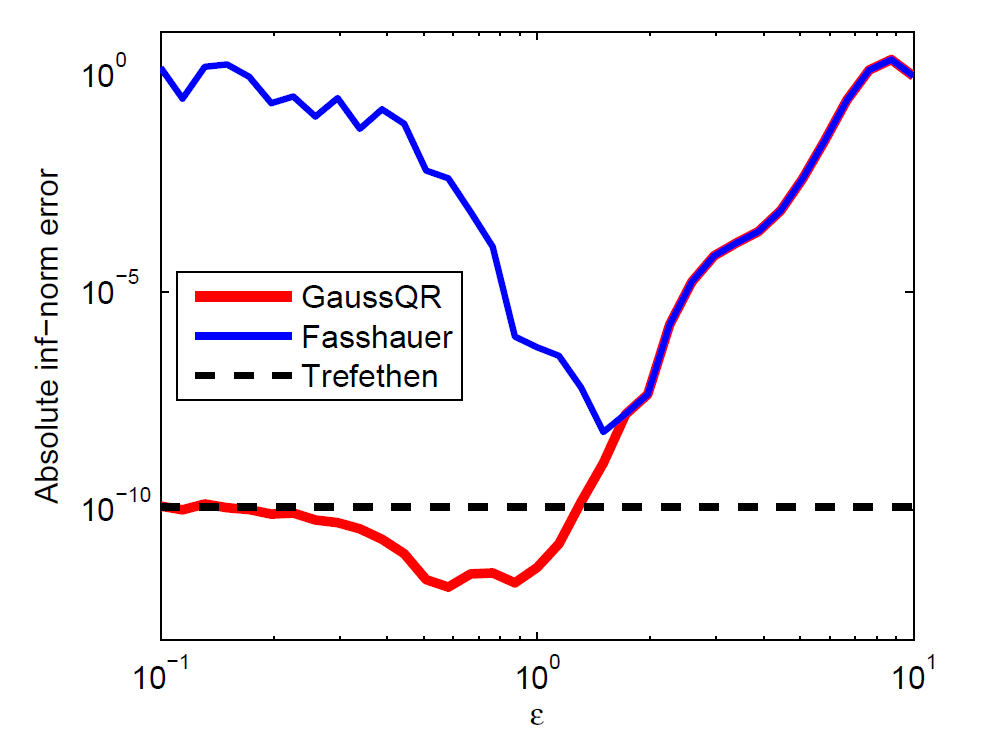
\includegraphics[height=2in]{HSSVD_BVP}
    \includegraphics[height=2in]{Fig_MFS_BEM}
\caption{Left: Comparison between use of the Hilbert--Schmidt SVD (GaussQR), standard kernel approach (Fasshauer) and Chebyshev polynomial spectral method (Trefethen) to solve a boundary value problem (from \citep{McCourt13}). Right: Cost per accuracy plot of several MFS solutions vs.\ BEM solution for coupled PDE system.}\label{Fig_MFS_BEM}
\end{figure}

As the next steps for this project we expect (i) to move to a head model that reflects the geometry of the brain more realistically, and (ii) to integrate the forward solver into a full inverse problem framework which will allow us to identify the locations of activity inside the brain from measurements of the electric potential (instead of simulating the electric surface potential based on a given dipole source as done for the forward problem in Fig.~\ref{Fig_MFS_BEM}).

\subsection*{Research Project 4.3. Using Kernels to Help Predict the Spread of Ebola} \label{ebolasubsec}
Mike McCourt is working on a project titled ``Modeling the Ebola Epidemic with Discrete Time Filters'' at UC--Denver, where the DEXES II software (developed for the analysis, planning, and training for complex international humanitarian emergencies, peacekeeping missions, and non-traditional conflicts) is being modified and then used to predict the state of the Ebola epidemic in West Africa within a data assimilation framework. A significant component of that work involves formalizing the mathematics of general discrete time filters, specifically the assimilation of data (assumed to be Poisson distributed), and implementing such a Poisson filter efficiently in software. Key quantities of interest (QoI) include: the probability of any cases developing in Mali, the probability of a multimodal evolution within a region (after an initial peak is hit, can the disease regain momentum), or the total number of cases outside of presently infected regions.
As an extension of that project, we plan to study the effect of various input parameters for 
the DEXES II model on the evolution of the Ebola crisis.  Such parameters may include: 
border permeability (the probability that someone can enter a country without screening), 
the development of quarantines within a region, and the availability of clean water and waste 
disposal facilities.  The QoI---computed at the end of a predictive session---may be written 
as QoI(permeability, quarantine, clean water) to denote its dependence on a variety of model 
parameters.  Studying the impact of these parameters on this QoI is a problem of surrogate 
modeling in potentially high dimensions.  Furthermore, as the number of dimensions we want 
to simultaneously consider increases, the experimental design for generating this surrogate 
model becomes increasingly relevant.  Thus, results from \refproba and \refprobcc should 
help with this Ebola study.



\section{Broader Impact of Proposed Research}\label{SectBroad}


\subsection{Contributions to Training, Mentoring and Other Human Resource Developments}

\begin{description}[leftmargin=0ex]
\item[Providing Research Experiences for Undergraduates and High School Students]\ We \linebreak[4]    strongly believe that students should be introduced to research before graduate school so that they can learn how to discover the unknown, something that is not taught well in a classroom. We request funds to support two summer REU students per year. Having advertised our REU opportunities for several years now has given us some visibility within the community and is prompting inquiries from prospective participants well before we even announce our latest program offerings. As in the past several years, we expect the NSF funds will serve as a catalyst for funds to support additional summer students. In choosing REU students we make a deliberate effort to build a diverse research environment by targeting female and underrepresented minority students as well as students from less research-focused institutions (see Sect.~\ref{SectPrevious}). We will also continue to receive well-prepared high school students to join our research group as we did for the past two summers.

\item[Preparing Students for Academic Careers] We consider mentoring to be a multi-faceted and potentially long-term process continuing even after the mentee has moved on from IIT.  For example, MM was an undergraduate student at IIT who collaborated with GEF during his PhD studies at Cornell U.  We will continue to mentor him as senior person for this proposal.
    %Similarly, although QY has left IIT, he has continued his collaboration with GEF and FJH.
    We have provided and will continue to provide SCC, a Research Assistant Professor at IIT and another senior person for this project, teaching and mentoring experience.  We will continue to find opportunities for special mentoring activities for our students, like those QY and YD participated in at the NSF-supported 14th International Conference on Approximation Theory in San Antonio organized by GEF in April 2013.  We  will continue our collaboration with Argonne National Laboratory, which has led to short-term and long-term opportunities for our PhD students and graduates.

\item[Preparing Students for Industry Careers]
In addition to preparing students for the academic landscape, we also help current students land competitive jobs in the business world. Our training in the areas of algorithm development and coding tends to give our students the needed edge. For example, WM graduated from Brown U in 2013 and then joined an internet startup company. AB, SD, YaL, and TS are working in the financial services industry.

\item[Supervising Visitors]
GEF has established contacts with several Italian universities attracting students and postdoctoral visitors to IIT for extended visits (see Sect.~\ref{SectPrevious}). Having lived in Hong Kong for 19 years, FJH has contacts with Chinese scientists that have prompted several long-term visiting Chinese scholars and students to join our research.  These activities will continue.

\item[Giving Short Courses and Invited Lectures]
We will continue our active track record of providing lectures to students at various stages in their careers, ranging from high school to graduate school. These encourage students to enter STEM and encourage STEM students to engage in research.

\end{description}

\subsection{Contributions to Resources in Research, Education and the Broader Society}

The research we propose straddles mathematics, statistics, computer science, and applications in engineering and related fields.  The two PIs have complementary strengths that facilitate this interdisciplinary research.  GEF has expertise in approximation theory, meshfree methods, and numerical PDEs, while FJH has expertise in (quasi-)Monte Carlo methods, kernel-based methods, information-based complexity theory, and experimental design. Our expertise provides both an obligation and an opportunity to interact with a number of diverse communities. We envision the following contributions:

\begin{description}[leftmargin=0ex]
\item[Disseminating Research]
The research supported by this grant will result in publications in peer-reviewed journals in a broad spectrum of applied mathematics, computer science, statistics and engineering. These journals will include both those that emphasize theory and those that emphasize applications.

\item[Promoting Cones] The idea of guaranteed, adaptive algorithms via cones of input functions has broad potential application.  We will be promoting this idea among numerical analysts who develop new algorithms and analyze their computational costs, as well as among information-based complexity theorists who analyze the lower bounds on the complexity of numerical problems.

\item[Promoting the Hilbert--Schmidt SVD] Similarly, we will encourage other researchers to take advantage of the stability given to kernel-based methods by the Hilbert--Schmidt SVD, to use our code, and to join our research efforts (\citep{FMcC12} has already more than 40 citations on Google Scholar).

\item[Bridging Mathematics and Statistics]
This project touches on topics that are of interest to the statistics community: kriging, Monte Carlo methods, and design of experiments.  Historically, there has been relatively little interaction between numerical analysts and statisticians.  We have and will continue to engage the statistics community by speaking a their conferences and departmental seminars.  For example, in 2015 FJH will give a colloquium talk in the Department of Statistics at Virginia Tech and an invited talk at the $47^{\text{th}}$ Days of Statistics of the Soci\'et\'e Fran\c{c}aise de Statistique. The book \citep{FMcC15} by GEF and MM will contain several chapters bridging this gap.

\item[Collaborating with Engineers]
GEF and MM have an ongoing collaboration with engineering colleagues at U Palermo (see \refprobdb). We have submitted two joint proposals to the Italian government and to U Palermo requesting support for our work (but without direct support for GEF and MM). Thus this collaboration will benefit from travel funds via the current proposal.
%Since kernel methods are becoming a rather popular numerical tool in science and engineering, other opportunities for collaborations outside mathematics frequently arise. For example, GEF participated in an incubator meeting on freeform surfaces organized by the Optical Society of America.

\item[Promoting the Well-being of the Broader Society]
\refprobdb uses kernel methods for the solution of inverse problems arising in the detection of brain activity from MEG or EEG data. This non-invasive diagnostic procedure might help doctors detect early functional and neurophysiological markers of diseases (e.g., Alzheimer's). It might also lead to a reduction in doctors' visits, shorter hospitalization periods and a greater longevity with overall improved quality of life. Similarly, \refprobdc may enable better management of the Ebola epidemic.

\item[Organizing and Presenting at Conferences]
We and our students involved in this project will present our results at a variety of conferences and workshops.  These include: (i) specialized meetings focusing on approximation theory, complexity, experimental design, meshfree methods, and Monte Carlo methods; (ii) the national meetings of AMS, SIAM, and the statistical societies; and (iii) conferences devoted to application areas.  We are frequently invited to speak at such conferences, which will give our results a prominent hearing. We will also continue to organize specialized conferences or minisymposia within larger conferences.

\item[Writing Textbooks and Survey Papers]
GEF and MM are currently preparing \citep{FMcC15}. This book will provide an exposition of the theory and implementation of the Hilbert--Schmidt SVD along with numerous applications. The book will form a bridge to the GaussQR library \citep{McCFBG13} and may serve as a textbook for a graduate class on meshfree methods, such as MATH 590 at IIT. GEF and FJH occasionally publish survey articles (e.g., a 42 page paper on kernel-based methods \citep{Fasshauer11}).

\item[Refreshing Course Syllabi]
MATH 590 (Meshfree Methods), taught by GEF in the fall semester of every even-numbered year, just underwent a major change as the preparation of \citep{FMcC15} progresses.
MATH 565 (Monte Carlo Methods in Finance), taught every fall by FJH, has incorporated our new results on guaranteed (quasi-)Monte Carlo multivariate integration. In the future it will include our new results on control variates and guaranteed multi-level and (quasi-)Monte Carlo sampling (see \refprobba).
Current texts teach students to estimate the error of the trapezoidal rule, $T_n(f)$, by $[T_n(f)-T_{n/2}(f)]/3$ (see, e.g., \cite[pp.\ 223--224]{BurFai10}).  The arguments behind this estimate introduce the valuable concept of extrapolation, however, this is a flawed error estimate as pointed out in \cite{Lyn83} and highlighted by our recent work \cite{HicEtal14b}.  This same flawed idea underlies \Matlab's {\tt integral.m}.  We will urge numerical analysis textbook authors and educators to change the way that error estimation is taught based on our recent and proposed work.  These ideas will also enter our more traditional numerical analysis courses such as MATH 350 (Intro to Computational Math) or MATH 577 and 578 (Computational Math I \& II).  SCC and FJH will continue to develop MATH 573 (Reliable Mathematical Software) as a valuable course for our own students and an example that we wish to propagate to other universities.

\item[Creating Software and Collaborating with Software Developers]
GEF and MM have created the website \citep{McCFBG13} which serves as the home for the software on our stable algorithms built upon the Hilbert--Schmidt SVD. This \Matlab library is freely available and allows others to experiment with our code. Thus far, the library contains routines for Gaussian and iterated Brownian bridge kernels. As our research expands to other kernels and their eigenexpansions the resulting code will be added to the library. The GaussQR library also serves as a sandbox for students---especially REU students---to learn about our research and allows them to contribute pieces of their own work.
We will continue to develop GAIL \citep{ChoEtal14a} (now up to version 2) as part of our proposed research.  The GAIL software will serve the wider community that relies on numerical approximation and integration algorithms.  It will also demonstrate how adaptive algorithms ought to be implemented, which we hope will inspire and inform those working on adaptive algorithms for other mathematical problems.  We also expect our new algorithms to be incorporated into widely used numerical packages, as was done for our algorithm in \cite{HonHic00a} by \Matlab \citep{MAT8.4} and NAG \citep{NAG23}.  We will continue to discuss with software developers about these issues.

\item[Reaching Out]
GEF and FJH both have a record of reaching out to high school students which we plan to continue. The website \href{http://math.iit.edu/~openscholar/meshfree/}{\nolinkurl{math.iit.edu/~openscholar/meshfree/}} helps manage our internal and external communication and dissemination of research findings. Advertising for the summer REU experiences is also facilitated via this website.  Information about GAIL is at \href{http://code.google.com/p/gail}{\nolinkurl{code.google.com/p/gail}}.
\end{description}

\newpage
\clearpage
%\pagenumbering{arabic}

\bibliographystyle{spbasic}

\renewcommand{\refname}{References Cited}                   %%
\renewcommand{\bibliofont}{\normalsize}

\bibliography{FJH23,FJHown23}
\end{document}
